\documentclass{../UTNetLab}

\title{Multicast and Realtime Service}
\authorshort{A. Khonsari, A. HajiAliKhamseh'i, M. Borhani, A. Khordadi, S. Kashipazha}
\author{%
    Dr. Ahmad Khonsari\\
    \FR{دکتر احمد خونساری}\\
    \mail{a\_khonsari@ut.ac.ir}
    \end{tabular}\vskip 1em
    \begin{tabular}[t]{c}
    Amir Haji Ali Khamseh'i\\
    \FR{امیر حاجی‌علی‌خمسه‌ء}\\
    \mail{khamse@ut.ac.ir}
    \and
    {Muhammad Borhani}\\
    \FR{محمد برهانی}\\
    \mail{m.borhani@ut.ac.ir}
    \and
    {AmirAhmad Khordadi}\\
    \FR{امیراحمد خردادی}\\
    \mail{a.a.khordadi@ut.ac.ir}
    \and
    {Sina Kashipazha}\\
    \FR{سینا کاشی‌پزها}\\
    \mail{sina\_kashipazha@ut.ac.ir}
    \and
    {Hadi Safari}\\
    \FR{هادی صفری}\\
    \mail{hadi.safari@ut.ac.ir}
    \and
    % {alii}\\
    % \FR{دیگران}\\
    % \mail{info@example.com}
}

\begin{document}
    \selectlanguage{english}
    \maketitle

\section*{Simple multicast exercises}
    For all the exercises in this section, the network topology is given in Fig.
    \ref{fig:fig13}\footnote{1.3 in Reference}, where all the hosts are connected to a single network segment using their default IP addresses, i.e.\  from 128.238.66.100 to 128.238.66.107.
    \begin{minipage}{0.48\textwidth}
        \begin{flushleft}
            \begin{table}[H]
                \caption{\textbf{Table 1.2} The IP addresses of the hosts}
                \label{tbl:1.2}
                \vspace{5pt}
                \centering
                \begin{tabular}{ l l l }
                    \hline \hline
                    Host & IP Address & Subnet Mask \\
                    \hline 
                    h0 (shakti) & 128.238.66.100 & 255.255.255.0 \\
                    h1 (vayu) & 128.238.66.101 & 255.255.255.0 \\
                    h2 (agni) & 128.238.66.102 & 255.255.255.0 \\
                    h3 (apah) & 128.238.66.103 & 255.255.255.0 \\
                    h4 (yachi) & 128.238.66.104 & 255.255.255.0 \\
                    h5 (fenchi) & 128.238.66.105 & 255.255.255.0 \\
                    h6 (kenchi) & 128.238.66.106 & 255.255.255.0 \\
                    h7 (guchi) & 128.238.66.107 & 255.255.255.0 \\
                    \hline \hline
                    \end{tabular}
            \end{table}
        \end{flushleft}
    \end{minipage}
    \begin{minipage}{0.48\textwidth}
        \begin{flushright}
            \begin{figure}[H]
                \centering
                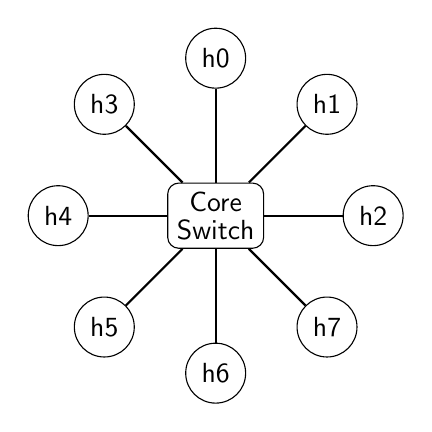
\begin{tikzpicture}[font=\sf]
                    \node[draw,rounded corners] (s) at (0,0){\shortstack{Core \\   Switch}};
                    \node[draw,circle] (h0) at (0,2){h0};
                    \node[draw,circle] (h1) at ({sqrt(2)},{sqrt(2)}){h1};
                    \node[draw,circle] (h2) at (2,0){h2};
                    \node[draw,circle] (h3) at (-{sqrt(2)},{sqrt(2)}){h3};
                    \node[draw,circle] (h4) at (-2,0){h4};
                    \node[draw,circle] (h5) at (-{sqrt(2)},-{sqrt(2)}){h5};
                    \node[draw,circle] (h6) at (0,-2){h6};
                    \node[draw,circle] (h7) at ({sqrt(2)},-{sqrt(2)}){h7};
                
                    \draw[thick] (h0) -- (s);
                    \draw[thick] (h1) -- (s);
                    \draw[thick] (h2) -- (s);
                    \draw[thick] (h3) -- (s);
                    \draw[thick] (h4) -- (s);
                    \draw[thick] (h5) -- (s);
                    \draw[thick] (h6) -- (s);
                    \draw[thick] (h7) -- (s);
                \end{tikzpicture}
                \caption{\textbf{Figure 1.3} A single segment network}
                \label{fig:fig13}
            \end{figure}
        \end{flushright}
    \end{minipage}

\section{Linux multicast routing table}
\label{sec:linux-multicast-routing}
    Execute \textbf{netstat -rn} to display the routing table of your host.
    If there is no entry for the 224.0.0.0 subnet, you need to provide a default route for multicast traffic, by:
    \begin{itemize}
        \item [] \textbf{route add -net 224.0.0.0 netmask 240.0.0.0 dev eth0}\footnote{This command can be appended to the \texttt{/etc/rc.local} file, so that it will be executed automatically when the system bootstraps. Each time when the network interface is brought down and up again by the \textbf{ifconfig} command, you may need to run the \textbf{route} command to re-insert the multicast routing entry.}
    \end{itemize}
    Save the new routing table.
    \subsection*{Report}
    Submit the routing table you saved.

\section{Multicast Membership}
    Execute \textbf{netstat -g} to show the multicast group memberships for all the interfaces in your host.
    \subsection*{Report}
    How many multicast groups did the interface belong to? What were the groups? Explain the meaning of the group IDs.

\section{Multicast Ping}
    Execute \textbf{ping 224.0.0.1}.
    Examine the \textbf{ping} output to see which hosts reply. \\
    Ping a broadcast address using \textbf{ping -b 128.238.66.255}.
    Examine the \textbf{ping} output to see which hosts reply. \\
    You can enable broadcast ping replay by: \textit{echo 0 > /proc/sys/net/ipv4/icmp\_echo\_ignore\_broadcasts}.
    \subsection*{Report}
    Which hosts replied when the multicast address was pinged?
    Which hosts replied when the broadcast address was pinged? \\
    In each case, was there a reply from your host?

\section{Multicast vs Unicast}
    Execute \textbf{tcpdump -n -nn -e} and \textbf{tcpdump ether multicast -n -nn -e} (or run \textbf{wireshark}) to capture an Ethernet unicast frame, an Ethernet multicast frame, and an Ethernet broadcast frame. \\
    To generate an Ethernet unicast frame, run \textbf{socket -i -u -n1} \textit{remote-host} \textbf{echo}. \\
    Execute \textbf{socket -i -u -n1 230.11.111.10 2000} to generate an Ethernet multicast frame. \\
    Generate another Ethernet multicast frame, but with a different group address of \texttt{232.139.111.10}. \\
    To generate an Ethernet broadcast frame, you may \textbf{ping} a remote host that has no entry in the ARP table of you host.
    Recall that the ARP request is broadcast. \\
    Save the frames captured for the lab report.

    \subsection*{Report}
    Compare the source and destination MAC addresses of the frames you captured. \\
    Use one of the multicast frames captured to explain how a multicast group address is mapped to a multicast MAC address.
    For the two multicast frames captured, do they have the same destination MAC address?
    Why?

\section{Simple UDP Multicast client and server}
    Start the multicast client \textbf{netspy} on all the hosts, by executing:
    \begin{itemize}
        \item [] \textbf{netspy 224.111.111.111 1500}
    \end{itemize}
    Then, start the multicast sender \textbf{netspyd} on \texttt{shakti}, by executing:
    \begin{itemize}
        \item [] \textbf{netspyd 224.111.111.111 1500 1}
    \end{itemize}
    Execute \textbf{tcpdump ip multicast} or \textbf{wireshark} on every host to capture multicast IP datagrams. \\
    Login to \texttt{shakti} from a remote machine, e.g.\  \texttt{kenchi}, using \textbf{telnet} or \textbf{ssh} (need to start ssh service). \\
    Save the captured multicast datagram sent by \textbf{netspyd} and exit the \textbf{telnet} (or \textbf{ssh}) session.

    \subsection*{Report}
    From the \textbf{tcpdump} output, how many messages are sent by \textbf{netspyd} when a new user logged in to \texttt{shakti}?
    From the \textbf{netspy} outputs on all the hosts, how many copies of the message are received in total? \\
    Did \texttt{shakti}, where the multicast sender, \textbf{netspyd}, was running, receive the multicast datagram?
    Why?
    If yes, through which interface did \texttt{shakti} receive this datagram?

\section{ping Replay}
    Enable broadcast ping replay by: \textit{echo 0 > /proc/sys/net/ipv4/icmp\_echo\_ignore\_broadcasts} on all hosts.
    Keep the \textbf{netspy} and the \textbf{tcpdump} programs running.
    Execute \textbf{ping 224.111.111.111} from \texttt{kenchi}.
    Examine the \textbf{tcpdump} and \textbf{ping} outputs to see which hosts replied.
    To avoid confusion, students should do this exercise by turns.
    Terminate the \textbf{netspy} programs on several hosts, e.g.\  \texttt{shakti}, \texttt{vayu}, and \texttt{fenchi}.
    Execute the \textbf{ping} command again.
    Also, examine the \textbf{tcpdump} and the \textbf{ping} outputs to see which hosts replied.

\section*{IGMP exercises}
    In the following exercises, use four hosts and one router. The network topology is given in Fig. 7.13, and the corresponding host IP addresses and router IP addresses are given in Table 7.2 and Table 7.3, respectively.

    \begin{table}[H]
		\caption{\textbf{Table 7.2.} Hosts IP addresses for Fig. 7.13}
		\label{tbl:7.2}
        \vspace{5pt}
        \centering
        \large
        \begin{tabular}{ *3l }
            \hline \hline
            Host & Name & Ip Address \\
            \hline
                host1 & shakti & 128.238.63.101/24 \\
                host2 & vayu   & 128.238.63.102/24 \\
                host3 & agni   & 128.238.64.103/24 \\
                host4 & apah   & 128.238.64.104/24 \\
            \hline \hline
            \end{tabular}
    \end{table}

    \begin{table}[H]
		\caption{\textbf{Table 7.3.} Router IP addresses for Fig. 7.13}
		\label{tbl:7.3}
        \vspace{5pt}
        \centering
        \large
        \begin{tabular}{ *3l }
            \hline \hline
            Host & eth0 & eth1 \\
            \hline
            router & 128.238.63.3/24 & 128.238.64.3/24 \\
            \hline \hline
            \end{tabular}
    \end{table}

    \begin{figure}[H]
        \centering
        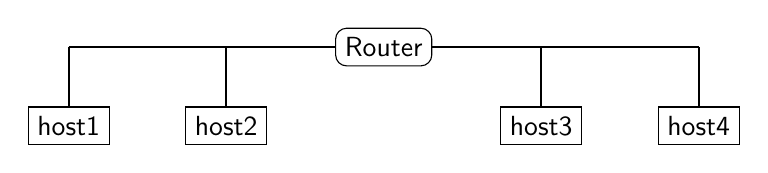
\begin{tikzpicture}[font=\sf]
            \node[draw] (h1) at (-4,-1){host1};
            \node[draw] (h2) at (-2,-1){host2};
            \node[draw,rounded corners] (router) at (0,0){Router};
            % \node[draw,rounded corners] (router) at (0,0){\shortstack{Router}};
            % \node[draw,circle] (hub1) at (2,0){Switch 1};
            \node[draw] (h3) at (2,-1){host3};
            \node[draw] (h4) at (4,-1){host4};
        
            \draw[thick] (h1) -- (-4,0);
            \draw[thick] (h2) -- (-2,0);
            \draw[thick] (h3) -- (2,0);
            \draw[thick] (h4) -- (4,0);
            \draw[thick] (4,0) -- (router);
            \draw[thick] (-4,0) -- (router);
        \end{tikzpicture}
		\caption{\textbf{Figure 7.13.} The network topology for the exercises in Section 7.5.}
		\label{fig:7.13}
    \end{figure}

\section{Configuring Router}
\label{sec:config-router}
    Connect the hosts and the route in your group as shown in Fig. 7.13. Set the IP address of your host as given in Table 7.2. Note that the IP addresses of the router interfaces are the same as their default IP addresses.
    Login to the router and run \textbf{ip multicast-routing} to enable multicast routing in the \textit{Global Configuration} mode.
    Then, enable the PIM protocol on each interface, by running \textbf{ip pim dense-mode} in the \textit{Interface Configuration} mode.\footnote{As usual,each router should be configured by one person to avoid confusion.} Now the router is enabled to do multicast routing using PIM. \\
    Login to the router, execute \textbf{show ip igmp interface} and \textbf{show ip igmp group} in the \textit{Privileged EXEC} mode.
    Examine the multicast group memberships currently recorded in the router and the configurations of the router interfaces.

\section{Multicast Message}
    Enable linux multicast routing in all the hosts (see \autoref{sec:linux-multicast-routing}).\\
    Start \textbf{netspy} on all the hosts, by using:
    \begin{itemize}
        \item [] \textbf{netspy 224.111.111.111 1500}
    \end{itemize}
    Start \textbf{netspy} on \texttt{host1} (\texttt{shakti}, by using:
    \begin{itemize}
        \item [] \textbf{netspyd 224.111.111.111 1500 16}
    \end{itemize}
    Login to the router.
    Run \textbf{show ip igmp interface} and \textbf{show ip igmp group} in the \textit{Privileged EXEC} mode again to examine the current membership records. \\
    Try if you can \textbf{ping} a host on the other side of the router.
    Login to \texttt{host1} from \texttt{host2} in your group, then logout.
    See if the multicast messages sent by \textbf{netspyd} reach the other side of the router.\\
    Add \texttt{route} for other subnet to your host and try \textbf{ping} again. Now, login to \texttt{host1} from \texttt{host2} in your group, then logout.
    \subsection*{Report}
    Can you ping a host on the other side of the router?
    Will the router forward a multicast IP datagram to the other side?
    Justify your answers.

\section{IGMP Types}
    Execute \textbf{tcpdump ip multicast -v} or \textbf{wireshark} in one console to capture IGMP messages.
    At the same time, execute \textbf{tcpdump ip multicast -v} in another console to monitor the capture process.
    When you see three or more IGMP queries in the second \textbf{tcpdump} output, terminate both \textbf{tcpdump} programs. \\
    Analyze the IGMP messages you captured.
    Print and save two different IGMP messages. \\
    Repeat the above experiment.
    Terminate \textbf{netspy} on \texttt{host2} and \texttt{host4}.
    Terminate the \textbf{tcpdump} programs and analyze the IGMP leave message you captured.
    \subsection*{Report}
    What is the value of the Time-to-Live (TTL) field for the IGMP messages?
    Why do we not set the TTL to a larger number? \\
    What is the default frequency at which the router sends IGMP queries?

\section{Router Join To Multicast-Group}
    Login to the router.
    See if you can make a router interface (e.g., Ethernet0) join a multicast group of 224.0.0.2, using:
    \begin{itemize}
        \item [] \textbf{ip igmp join-group 224.0.0.2}
    \end{itemize}
    \subsection*{Report}
    Explain why the above command fails.

\section*{Multicast routing exercises}
    For the rest of the exercises in this chapter, the network topology is given in Fig. 7.14. The exercises will be jointly performed by all the students. The IP addresses of the hosts and router interfaces are given in Fig. 7.14.
    \begin{figure}[H]
        \centering
        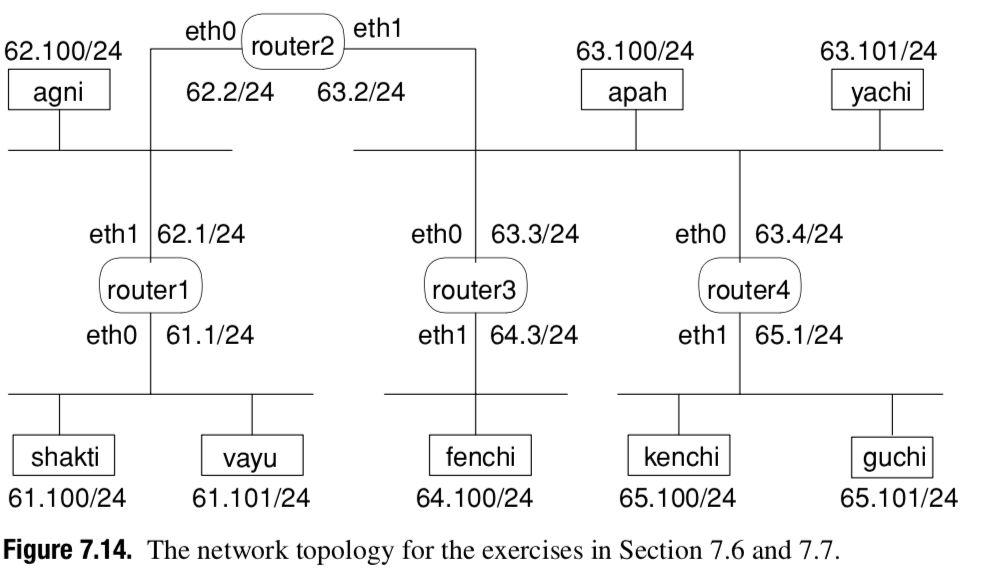
\includegraphics[width=0.9\textwidth]{img/figure7-14.png}
        \label{fig:7.14}
    \end{figure}

\section{Multicast Multi-Hub}
    Connect the hosts and routers as illustrated in Figure 7.14.
    Configure the IP addresses of the hosts and router interfaces as given in the figure.\\
    % Note that most of the router interfaces use their default IP addresses, only the Ethernet0 interface of Router4 needs to be changed to 128.238.63.4. \\
    Enable linux multicast routing in all the hosts (see \autoref{sec:linux-multicast-routing}).\\
    Enable PIM multicast routing in all the routers (see \autoref{sec:config-router}). \\
    Run \textbf{tcpdump ip multicast} or \textbf{wireshark} on all the hosts. \\
    Execute \textbf{netspy 224.111.111.111 1500} on \texttt{shakti, agni, apah, fenchi}, and \texttt{kenchi}.
    Execute \textbf{netspyd 224.111.111.111 1500 16} on \texttt{yachi}.
    To generate multicast traffic, you can login (by \textbf{telnet} or \textbf{ssh}) to or logout of \texttt{yachi}.
    Each time when the login user set of \texttt{yachi} changes, \textbf{netspyd} on \texttt{yachi} will send a multicast datagram to group 224.111.111.111, to report the change in its login users. \\
    Can you see the \textbf{netspy} messages on the 128.238.65.0 (or the 128.238.61.0) subnet in the \textbf{tcpdump} output? \\
    Terminate the \textbf{netspy} program on \texttt{kenchi} (or \texttt{shakti}).
    Can you see the \textbf{netspy} messages on the 128.238.65.0 (or the 128.238.61.0) subnet?
    \footnote{If IGMPv1 is used, a participant does not send a leave message when it leaves the group.
    In this case, the membership record in the router expires in 120 seconds.
    During this interval, the router still forwards multicast datagram through the port.} \\
    Save one of the PIM routing packets.
    You may use \textbf{tcpdump} output to analyze it.
    What is the destination IP address used in this PIM routing packet?
    \subsection*{Report}
    Answer the above questions.

\section{Multicast tree}
    In this exercise, try the \textbf{mstat} Cisco IOS command to find the multicast tree from a source.
    The \textbf{mstat} command is executable in the \textit{Privileged EXEC} mode.
    You can always type “?” to get help on the syntax of the command.\\
    \textit{generate multicast packet when execute command for specific source}

\section{Multicast TTL}
    Keep \textbf{netspy} running on all the hosts.
    Ping the multicast group address from yachi, using: \\
    \textbf{ping 224.111.111.111 -t} \textit{n} \\
    The parameter \textit{n} is the TTL to be set to the multicast datagrams sent by ping.
    Try different values of \textit{n}, e.g.\  1, 2, 3, and 16.
    See how far a multicast datagram can travel with different TTL values. \\
    Now, login to \texttt{Router2}, in the \textit{Interface Configuration} mode, set the TTL threshold of the \texttt{Ethernet0} interface to 32, using: \\
    \textbf{ip multicast ttl-threshold 32}
    \footnote{The syntax of this command may be different for different versions of CiscoIOS. You may use“?” to get help.} \\
    Run the \textbf{ping} command with \textit{n} = 16 again.
    Can you see the multicast datagrams in the 128.238.61.0 and 128.238.62.0 subnet?
    Try \textit{n} = 33.
    Answer the same question.
    \subsection*{Report}
    Answer the above questions. \\
    What is the use of the TTL threshold in the router interface?

\section*{Multicast video streaming exercise}
    In the following exercise, we use \textbf{vlc} for video streaming.
    The routers and hosts have the same configurations as in Fig. 7.14.

\section{Multicast Real-Time Video}
    Start \textbf{vlc} on all the hosts, by using \textbf{vlc \&}. \\
    On \texttt{shakti}, go to the \textbf{vlc} menu: \texttt{Media/Stream \ldots }. Chose video file \texttt{/home/netlab/group.mp4} and press “stream” button. In “Stream output” add “RTP /MPEG Transport Stream” dialog.
    Then click the “next” button.
    In the next window, specify the multicast group address to be \textbf{224.123.111.101}, with port number \textbf{22224} %and TTL 33.
    Then click the “Finish” button.
    Now the \textbf{vlc} on \texttt{shakti} is transmitting the video clip using \texttt{RTP/RTSP/UDP/IP} to the multicast group \textbf{224.123.111.101} on port \textbf{22224}. \\
    On all other hosts, go to the \textbf{vlc} menu: \texttt{Media/Open Network Stream \ldots.} In the following “Open RTP Session” dialog, specify the same group address, port number as that used in \texttt{shakti}.%and TTL
    Now you should see the received video is displayed on the screen. \\
    Execute \textbf{tcpdump ip multicast} or \textbf{wireshark} in one console to capture the multicast datagrams.
    In another console, execute \textbf{tcpdump ip multicast} to monitor the capture process.
    When you see some \texttt{RTCP} packets in the second \textbf{tcpdump} output, terminate both \textbf{tcpdump} programs. \\
    Analyze the header format of a \texttt{RTP} data packet and a \texttt{RTCP} Sender (or Receiver) Report packet.


    \appendix
\section*{Appendices}
\addcontentsline{toc}{section}{Appendices}
\renewcommand{\thesubsection}{\Alph{subsection}}

\subsection{Configuring a multicast router}
\textit{The \textbf{no} form of this command cancels the group membership}
\subsubsection{Configuring IGMP}
\begin{itemize}
    \item ip igmp join-group group-address
    \item no ip igmp join-group group-address
    \item ip igmp query-interval \textit{new-value-in-seconds}
    \item no ip igmp query-interval
    \item show ip igmp groups: \textit{Displays the multicast groups in the attached
    networks.}
    \item show ip igmp interface: \textit{Displays multicast related information on a
    router interface.}
    \item debug ip igmp: \textit{Displays IGMP packets received and transmitted.}
\end{itemize}

\subsubsection{Configuring multicast routing}
\begin{itemize}
    \item ip multicast-routing
    \item no ip multicast-routing
    \item ip pim [dense-mode | sparse-mode | dense-sparse-mode].
    \item show ip mroute: \textit{Displays the multicast routing table.}
    \item show ip mroute summary: \textit{Displays a one-line summary for each entry in the multicast routing table.}
    \item show ip mroute count: \textit{Displays multicast statistics.}
    \item show ip dvmrp route: \textit{Displays the DVMRP routing table.}
    \item show ip pim neighbor: \textit{Lists PIM neighbors discovered by the router.}
    \item show ip pim interface: \textit{Displays router interface configurations.}
\end{itemize}

\subsubsection{Cisco IOS multicast diagnostic tools}
\begin{itemize}
    \item mtrace
    \item mrinfo
    \item mstat
    \item ping
\end{itemize}

\end{document}